\documentclass[conference]{IEEEtran}

% *** GRAPHICS RELATED PACKAGES ***
%
\ifCLASSINFOpdf
\usepackage[pdftex]{graphicx}

\hyphenation{op-tical net-works semi- -tor}

\begin{document}
\title{Synthesis of sound with nodes}

% make the title area
\maketitle

\begin{abstract}
%\boldmath
This project aims to create a tool for computer sound synthesis by only using nodes, which can be placed on a canvas and connected with wires.
The main objective of the project is to create a tool for learning computer sound synthesis without the need for programming.
\end{abstract}

\IEEEpeerreviewmaketitle

\section{Introduction}
Computer sound generation became the norm in the current era of entertainment industries.
Game, movie, music, and other industries have all adopted the computer sound generation, and practically all of the products these industries produce use some form of computer sound generation.
This project's main objective is to implement a tool for computer sound synthesis with visual programming.
The application's main goal is to help users learn the basics of computer sound generation without the need for programming.
Figure \ref{fig:example-node-based-audio-synth} shows an example tool for a node-based audio synth.

\section{Goals}
The main goal of this project is the implementation of a tool for computer sound synthesis with visual nodes instead of the usual programming approach.
The tool will provide a collection of nodes for sound generation, i.e., sine wave generator, file input; nodes for sound manipulation, i.e., adder, multiplier, passthrough, filters; and for sound output, i.e., players, file writers, and others.
The user will be able to place the nodes on a canvas and connect them with a wire, resulting in a transfer of data from the output of a node to the input of another node.
The tool's main objective is to improve the learning process of computer sound generation without the need for programming, which requires an intuitive and easy-to-use interface.
\begin{figure}
\centering
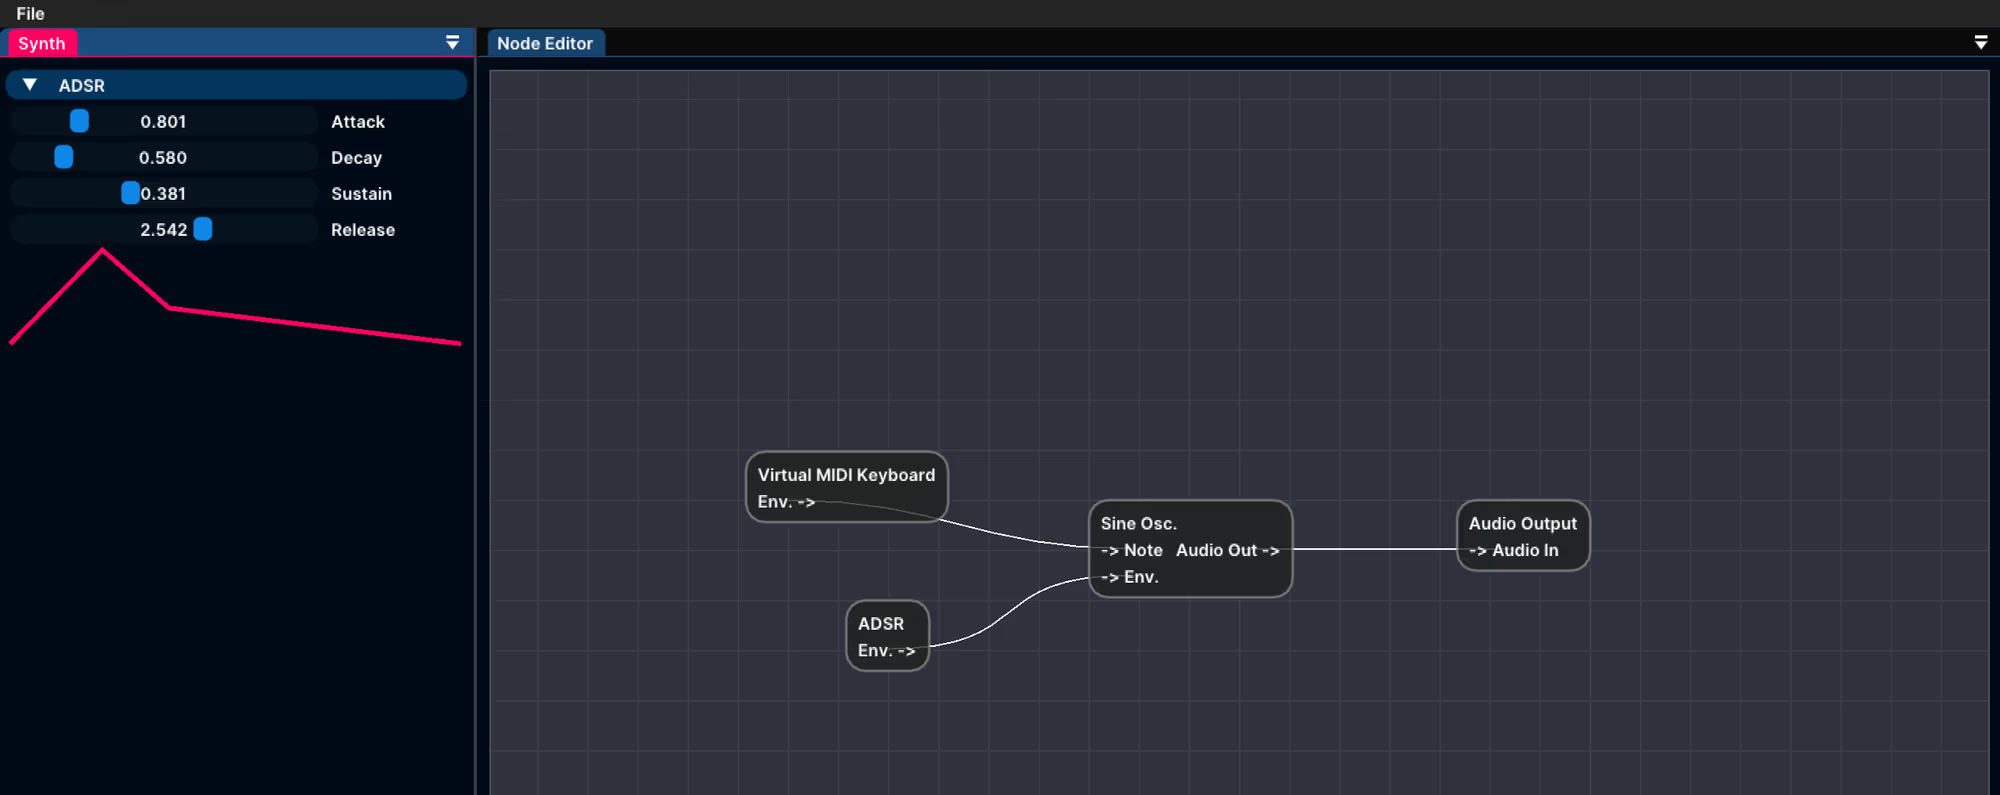
\includegraphics[width=1.0\linewidth]{graphics/example-node-editor.png}
\caption{A similar project Node-Based Audio Synth \cite{nodebasedaudiosynth}, implemented in C++ programming language. The image displays a simple UI with a couple nodes that generate sound.}
\label{fig:example-node-based-audio-synth}
\end{figure}

\section{Implemetaion}
The main programming language used in this project will be C++.
For the input and output of sound, RtAudio~\cite{rtaudio}, a lightweight, cross-platform API (Application Programming Interface) for realtime audio input and output, will be used.
UI (User Interface) will be implemented using an open source library ImGui~\cite{imgui} for creation of GUIs (Graphical User Interfaces) in C++ in combination with ImGui Node Editor~\cite{imguinodeeditor}, a node editor implementation.

The end product will give the user a collection of nodes used to generate, manipulate, and output a sound. The node collection will be heavily inspired by the one provided with the Java API JSyn~\cite{jsyn}.
Example nodes are: sine wave generator, adder, multiplier, passthrough, different filters, and a standard output node.
Those nodes will have inputs and outputs, defined with so-called \textbf{pins}, which are connected with \textbf{wires}.
The user will be given the power to instantiate the node on a canvas and connect an output to an other node's input with a wire.
With this process, any sound synth can be produced.

First, we will implement individual components (sine wave generator, adder, etc.) in C++ and define an API for creation, deletion, and connecting of those components. Then, we will use the API to implement a user interface with ImGui Node Editor~\cite{imguinodeeditor}.

Another feature of the tool will allow the users to implement their own nodes with extensions of the base classes provided with the API.

\section{Evaluation}
The solution will be evaluated with the help of JSyn~\cite{jsyn}. The same synth will be assembled in both tools and the output compared by looking at the raw data and by listening to the sound. The implemented tool will be evaluated based on the deviation in the data.

The performance will be tested in a similar way. Both tools will be used to create the same synth, and the time of synthesization will be measured.

\begin{thebibliography}{1}
\bibitem{jsyn}
JSyn:~API for developing interactive sound applications in Java https://www.softsynth.com/jsyn/

\bibitem{rtaudio}
RtAudio:~API for realtime audio input/output in C++ https://www.music.mcgill.ca/~gary/rtaudio/

\bibitem{nodebasedaudiosynth}
Node-Based Audio Synth https://eilu.me/en/portfolio/node-based-audio-synth/

\bibitem{imgui}
ImGui:~API for GUI in C++ https://github.com/ocornut/imgui

\bibitem{imguinodeeditor}
Imgui Node Editor:~Implementation of a node editor using ImGui https://github.com/thedmd/imgui-node-editor

\end{thebibliography}

\end{document}